% ACH1 project
% Fridolin Pokorny
% xpokor32@stud.fit.vutbr.cz
% date: 30.09.2013

\documentclass[11pt,a4paper]{article}
\usepackage[slovak]{babel}
\usepackage[top=2.5cm, left=2cm, right=2cm, text={18cm, 25cm}]{geometry}
\usepackage[T1]{fontenc}
\usepackage[utf8]{inputenc}

\newcommand{\uva}[1]{\quotedblbase #1\textquotedblleft}

\usepackage{xcolor}%[usenames,dvipsnames]
%\usepackage{listings,fancyvrb,multicol,array}
%\usepackage{pdflscape}

\usepackage{caption}
\DeclareCaptionFont{white}{\color{white}}
\DeclareCaptionFormat{listing}{\colorbox{gray}{\parbox{0.988\textwidth}{#1#2#3}}}
\captionsetup[lstlisting]{format=listing,labelfont=white,textfont=white}
\usepackage{titlesec}
%\usepackage[colorinlistoftodos]{todonotes}
\usepackage{xcolor}
\usepackage{longtable}
\usepackage{verbatim}
\usepackage{color}
\usepackage{hyperref}
\usepackage{textcomp}
\usepackage{graphicx}
\usepackage{float}
%\usepackage{wrapfig}
%\usepackage{siunitx}
\usepackage{lipsum}
%\usepackage{amsmath}
\usepackage{lscape}
\usepackage{fancyvrb,parcolumns}
\titleformat{\chapter}
  {\normalfont\LARGE\bfseries}{\thechapter.}{1em}{}

\definecolor{col_ident}{RGB}{10,10,90}
\definecolor{col_keyw}{RGB}{160,0,0}
\definecolor{col_comm}{RGB}{0,80,0}
\definecolor{col_str}{RGB}{255,127,0}

\definecolor{col_obj_addr}{RGB}{0,0,0}
\definecolor{col_obj_insn}{RGB}{90,90,40}
\definecolor{col_obj_cnst}{RGB}{0,0,0}
\definecolor{col_obj_othr}{RGB}{255,127,0}

\begin{document}
\title{Dokumentácia projektu do kurzu Biometrické systémy}
\author{Pokorný Fridolín \& Tomáš Rajca}
\date{\today}

\vspace*{\fill}
\begin{center}
\textbf{\Huge\textbf{Dokumentácia projektu do kurzu Biometrické systémy}} \\
\vspace{8mm}
\textit{\Large\color{gray} Rozpoznání žil prstu}\\
\vspace*{\fill}
\vspace*{\fill}
\hfill\textbf{Pokorný Fridolín} \\
\hfill{\href{mailto:xpokor32@stud.fit.vutbr.cz}{\nolinkurl{xpokor32@stud.fit.vutbr.cz}}} \\
\hfill\textbf{Rajča Tomáš} \\
\hfill{\href{mailto:xrajca00@stud.fit.vutbr.cz}{\nolinkurl{xrajca00@stud.fit.vutbr.cz}}} \\
\hfill{FIT VUT Brno} \\
\hfill\today
\end{center}
\vspace*{\fill}

\renewcommand{\baselinestretch}{1.5}
\thispagestyle{empty}
\clearpage

\begin{verbatim}
TODO:
  * popisat Alg3 + vysledky
  * popisat Alg4 + vysledky
  * popisat Alg5 + vysledky
\end{verbatim}

\setcounter{page}{1}
\clearpage

\section{Úvod} \label{uvod}

Tento dokument popisuje prístupy a metódy použité pri práci na projekte do kurzu
Biometrické systémy. Cieľom projektu bolo implementovať a otestovať algoritmus
pre rozpoznávanie ľudí na základe žíl na prstoch pomocou
\emph{BIO.Framework}\,--\,u. V práci je možné nájsť analýzu niekoľkých
implementovaných algoritmov spolu s ich vyhodnotením a stručným popisom.
Implementačné detajly je možné následne nájsť v priložených zdrojových súboroch.

Dokumentácia je členená na niekoľko častí. V časti \ref{data} je možné nájsť
informácie o použitých obrazoch zo senzora spolu s ukážkami a ich analýzou. Časť
\ref{algoritmy} sprehľadňuje jednotlivé navrhnuté a implementované algoritmy.
V tejto sekcii je možné nájsť aj prehľad výsledkov algoritmov v ucelenom
porovnaní. Časť \ref{konalio} analyzuje výsledky existujúceho nástroja. Posledná
časť \ref{zaver} sumarizuje výsledky práce.

\section{Vstupné data} \label{data}

Vstupné data tvorili poskytnuté snímky zo senzorov. Ukážku použitých snímkov je
možné vidieť na obrázkoch v ukážke \ref{fig:img}. 

\begin{figure}[ht!]
	\centering
	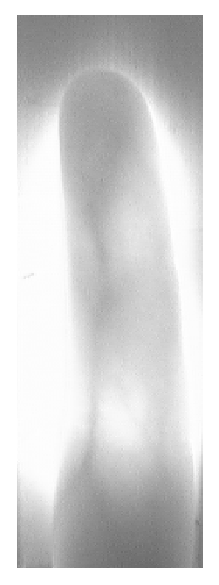
\includegraphics[width=2.5cm]{fig/img1.eps}
	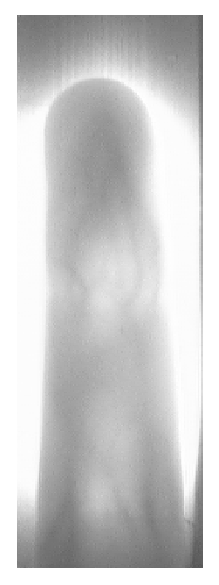
\includegraphics[width=2.5cm]{fig/img2.eps}
	\caption{\label{fig:img} Ukážka snímkov zo senzorov}
\end{figure}

Snímky boli uložené ako obrazové bitmapy vo formáte BMP s výškou 119 a šírkou
354 pixelov. Farebná hĺbka snímkov bola 24bitov, snímky však boli pravdepodobne
predspracované, šedotónové.

Celkovo bolo použitých 126 snímkov od 7 ľudí, každý človek teda poskytol 18
rôznych snímkov rovnakého prstu z rovnakej ruky.

Bežným ľudským okom bolo presné rozpoznanie zo snímkov veľmi obtiažne,
v niektorých prípadoch až nemožné.

\section{Implementované algoritmy} \label{algoritmy}

V tejto sekcii je možné nájsť návrh, analýzu a vyhodnotenie jednotlivých
implementovaných algoritmov pre rozpoznanie človeka na základe žíl prstu.

\clearpage
\subsection{\emph{Alg1}\,--\,porovnanie hodnôt pixelov} \label{alg1}

Prvý implementovaný algoritmus pozoruje hodnoty jednotlivých pixelov, ktoré
porovnáva. Tento algoritmus nie je nijak špeciálne sofistikovaný. Zámer jeho
implementácie bolo jeho využitie pre postupné rozširovanie a porovnávanie
zlepšení voči prostému porovnaniu hodnôt pixelov. Ako je vidieť na obrázku
\ref{fig:alg1}, algoritmus nevykazuje výsledky vhodné pre rozpoznanie, preto
cieľom ďalších algoritmov bude zlepšiť tieto výsledky a porovnať výsledok
s týmto referenčným riešením.

\vfill
\begin{figure}[ht!]
	\centering
	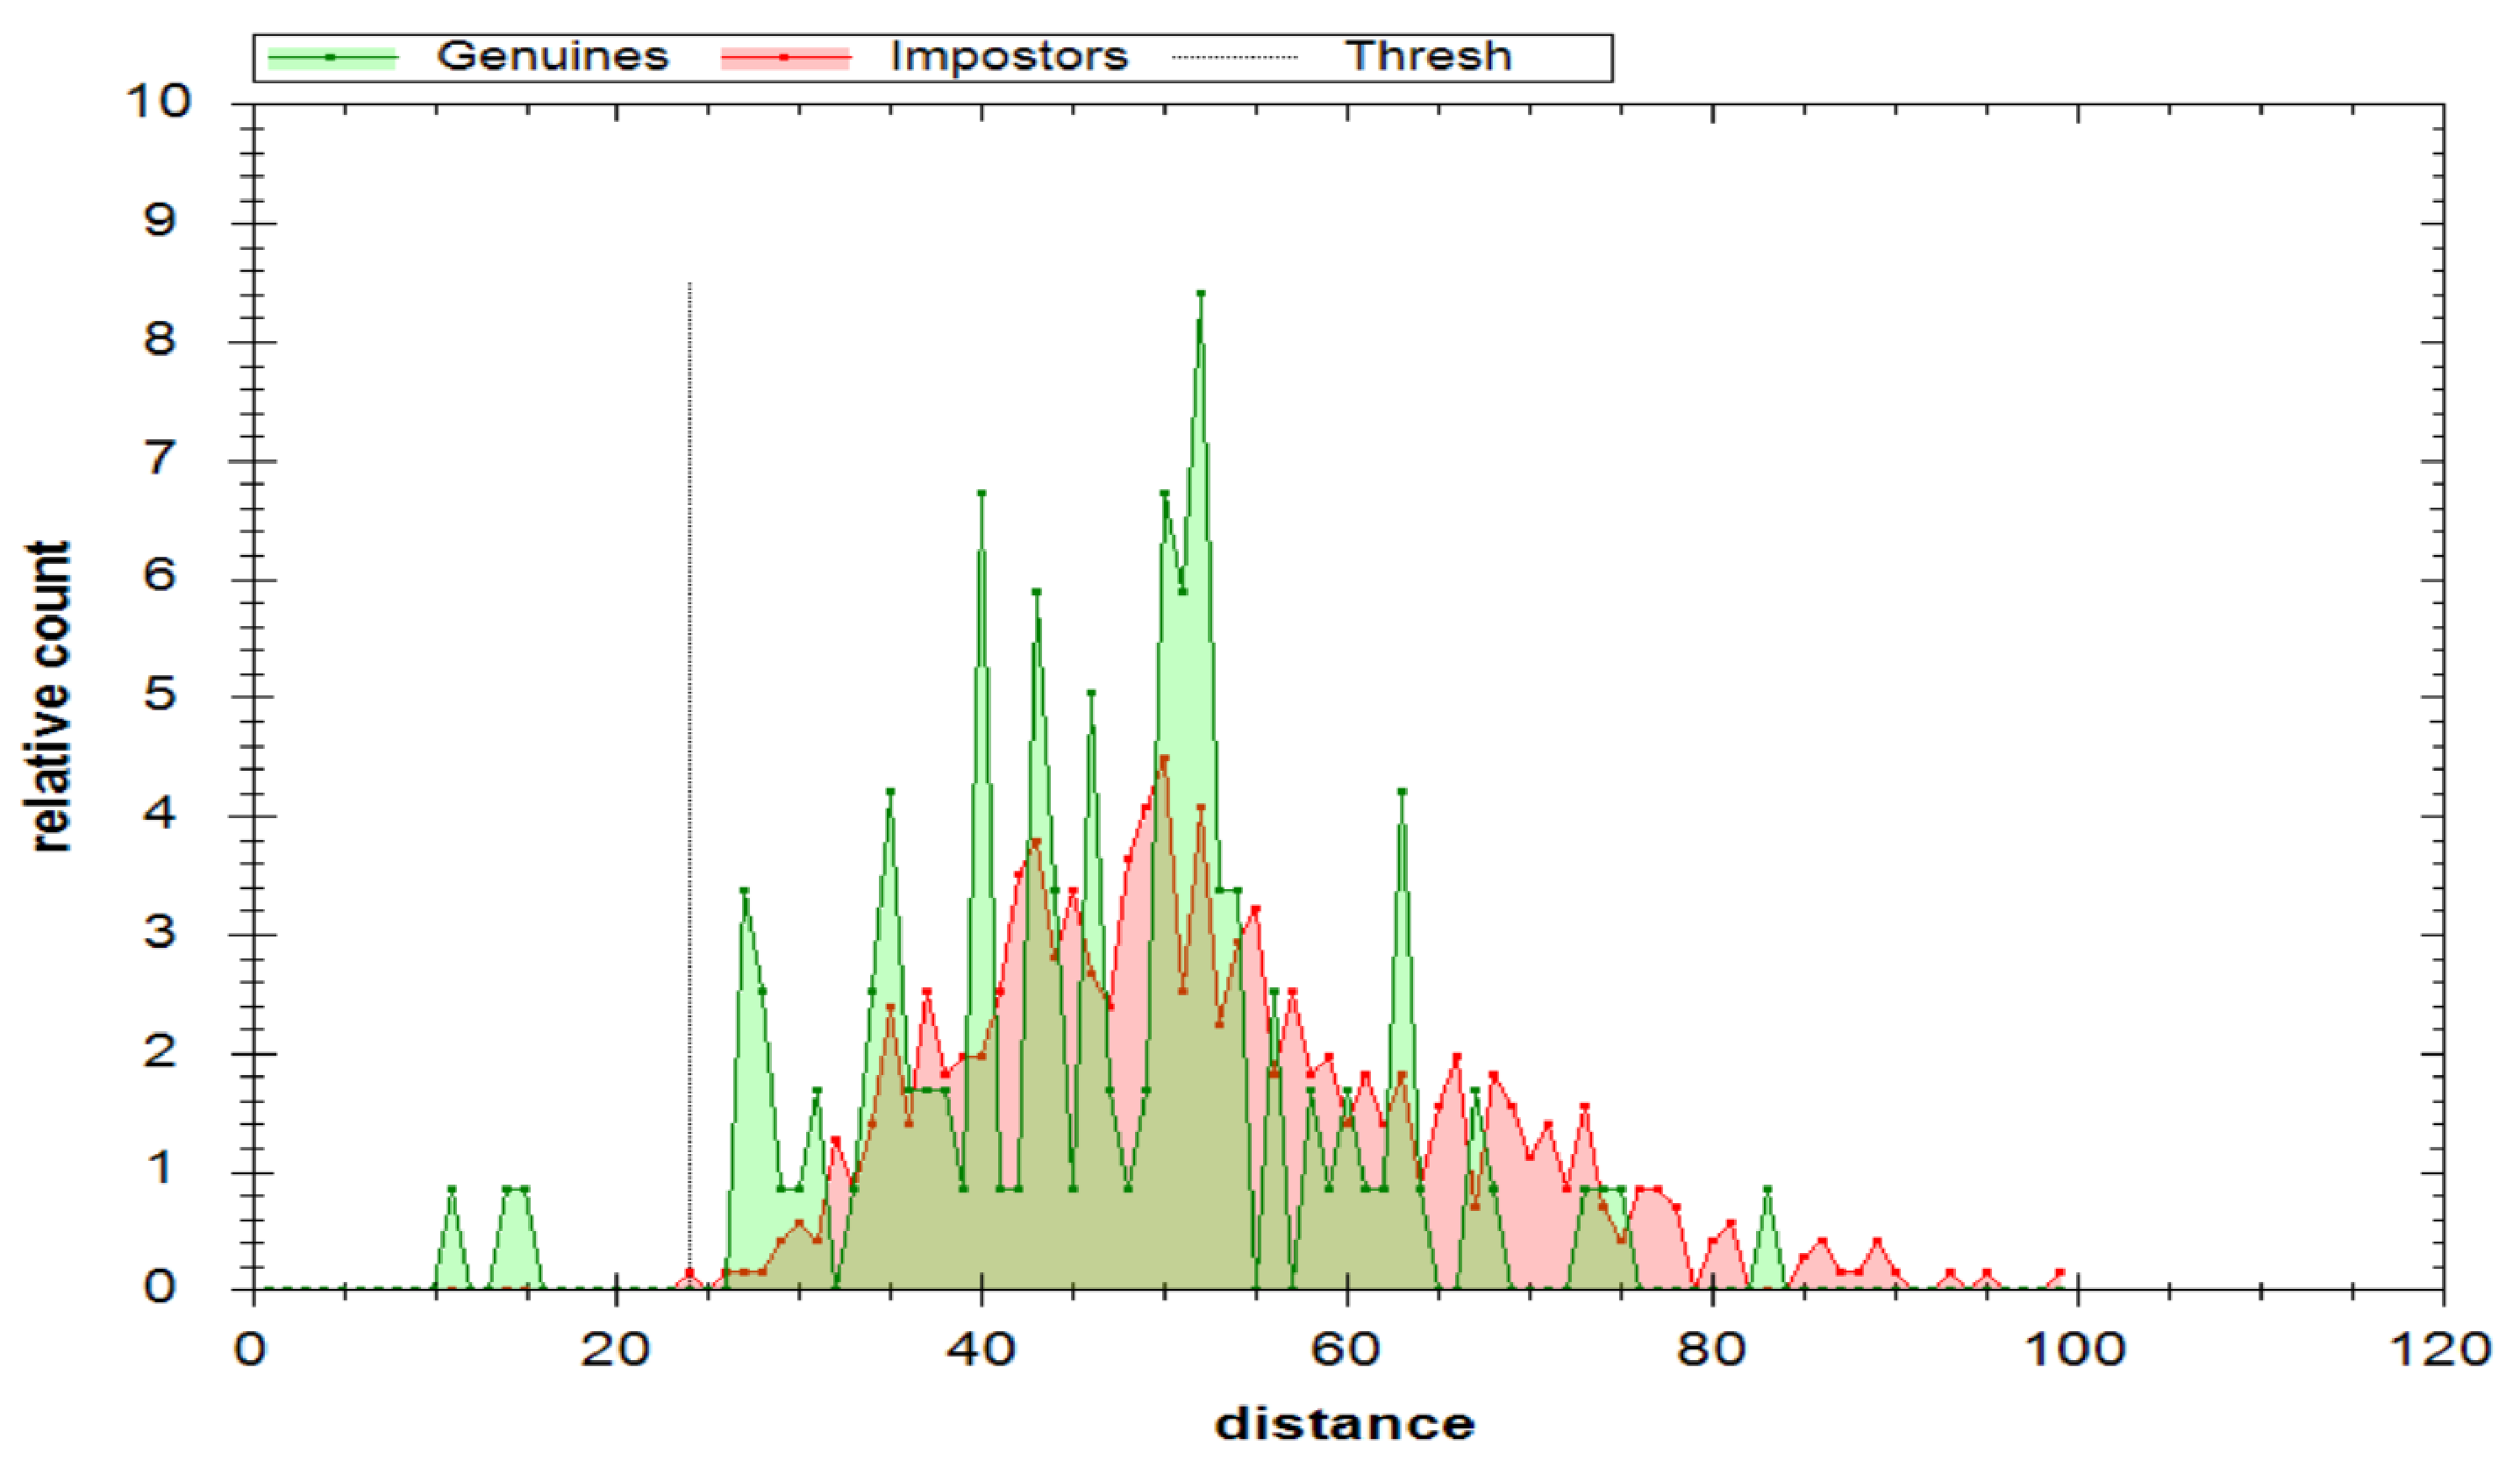
\includegraphics[width=17cm]{fig/alg1.eps}
	\caption{\label{fig:alg1} Výsledky implementovaného algoritmu \emph{Alg1}}
\end{figure}
\vfill
\vfill

\clearpage
\subsection{\emph{Alg2}\,--\,úprava histogramu} \label{alg2}

V poradí druhý implementovaný algoritmus využíva okrem porovnanie hodnôt pixelov
aj úpravu hodnôt pixelov vzhľadom na histogram. Obrázok \ref{fig:alg2}
demonštruje výsledky implementovaného algoritmu. Je možné vidieť zlepšenie
rozpoznania v porovnaní s prvým implementovaným algoritmom, avšak výsledky
algoritmu nie sú požiteľné pre reálne nasadenie.

\vfill
\begin{figure}[ht!]
	\centering
	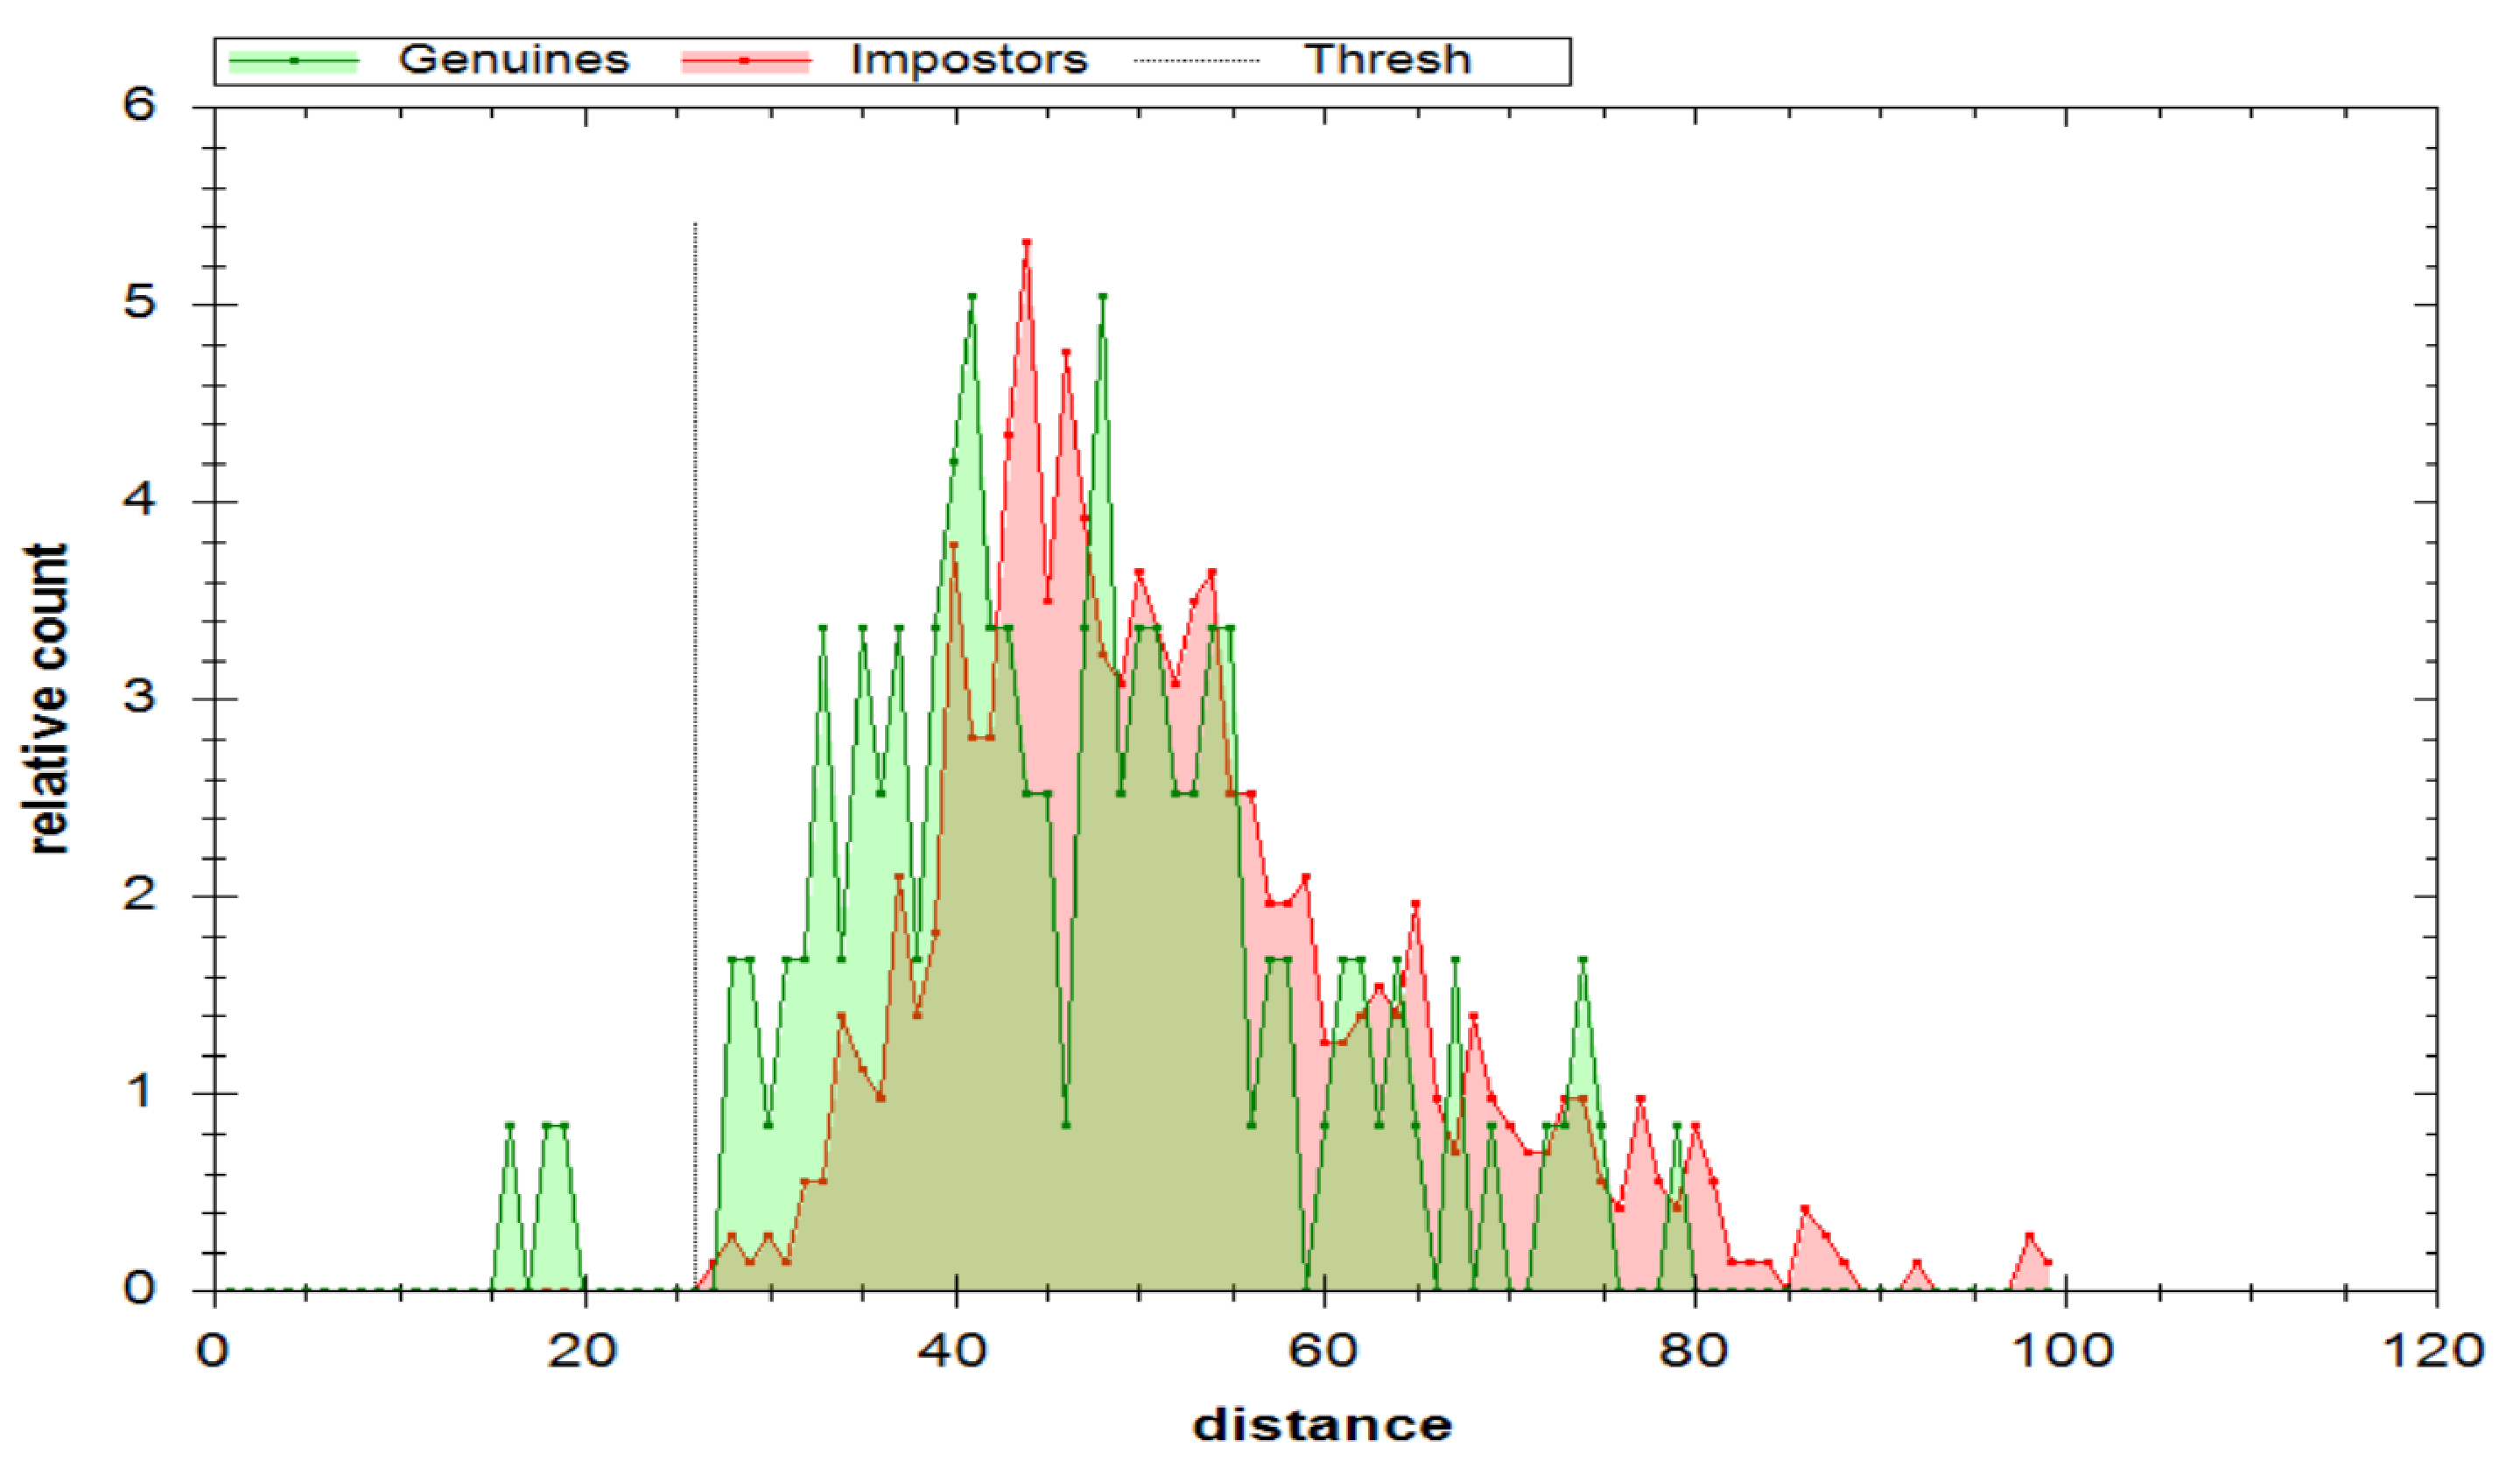
\includegraphics[width=17cm]{fig/alg2.eps}
	\caption{\label{fig:alg2} Výsledky implementovaného algoritmu \emph{Alg2}}
\end{figure}
\vfill
\vfill

\clearpage
\subsection{\emph{Alg3}\,--\,orezanie vstupného snímku} \label{alg3}

Tretí algoritmus sa snažil rozpoznať prst na vstupnom snímku a orezať vstupný
snímok tak, aby nedochádzalo k porovaniu pozadia snímku - lampy a tieňov.
Výsledkom extrakcie teda mohli byť obecne rôzne veľké snímky, ktoré obsahovali
orezanú časť vstupného obrázku. Pri porovnávaní sa následne prispôsobila veľkosť
porovnávaných obrázkov menším rozmerom (porovnávanie s väčšími pri použití
lineárnej interpolácie nemalo zásadnejší vplyv na výsledky).

Ukážka orezaného vstupného snímku je ilustrovaná na príklade \ref{fig:alg_out}.
Výsledky algoritmu sú prezentované v grafe \ref{fig:alg3}. Celkovo sa
rozpoznávanie nezlepšilo, v niektorých prípadoch došlo skôr ku skôr zhoršeniu.

\vfill
\begin{figure}[ht!]
	\centering
	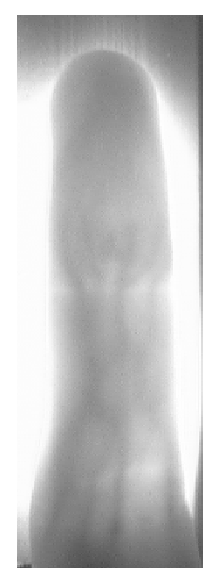
\includegraphics[height=5cm]{fig/alg3_in.eps}
	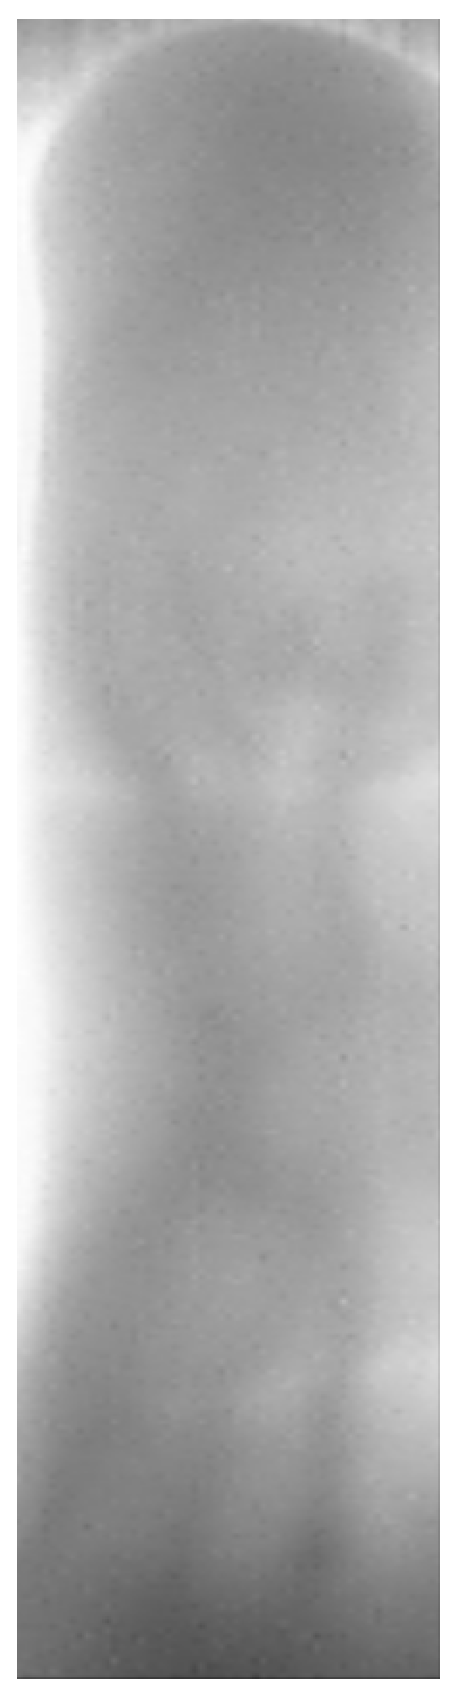
\includegraphics[height=5cm]{fig/alg3_out.eps}
	\caption{\label{fig:alg_out} Príklad orezania snímku tretím algoritmom}
\end{figure}

\vfill

\begin{figure}[ht!]
	\centering
		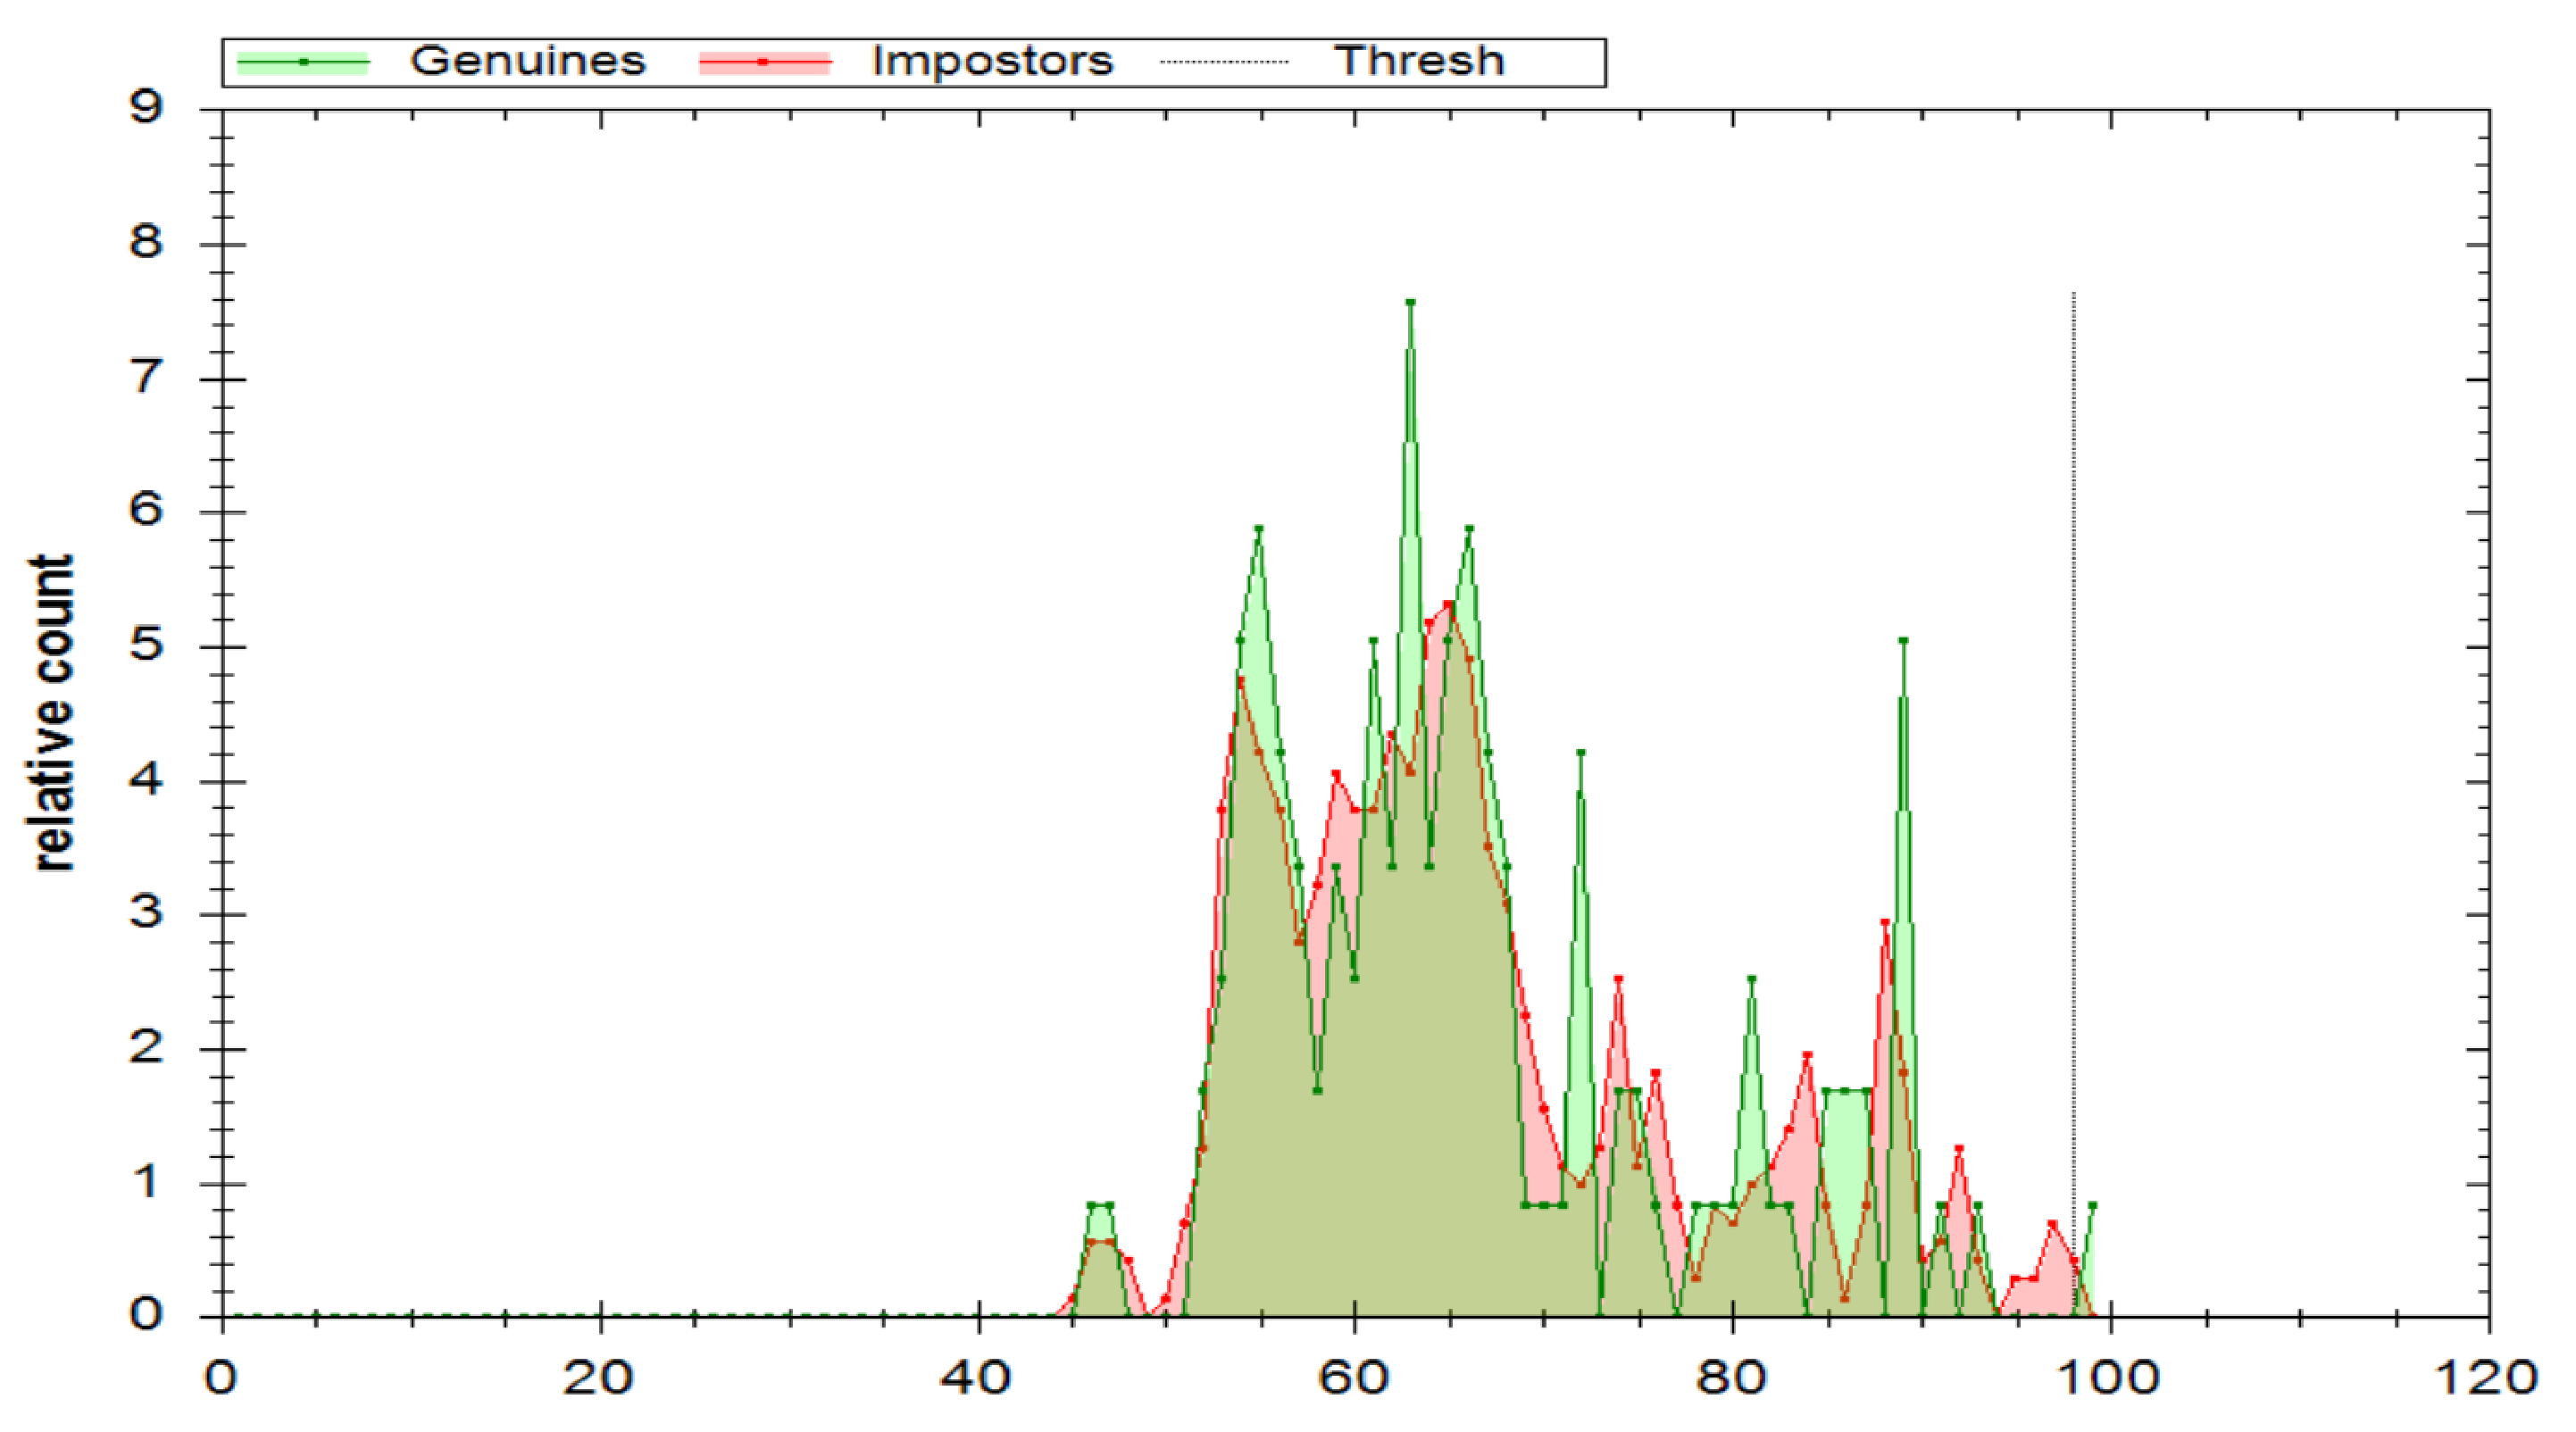
\includegraphics[width=17cm]{fig/alg3.eps}
	\caption{\label{fig:alg3} Výsledky implementovaného algoritmu \emph{Alg3}}
\end{figure}
\vfill

\clearpage
\subsection{\emph{Alg4}\,--\,} \label{alg4}
\texttt{TODO}
\lipsum[1-32]

\begin{figure}[ht!]
	\centering
	
\includegraphics[width=12cm]{fig/alg4.eps}
	\caption{\label{fig:alg4} Výsledky implementovaného algoritmu \emph{Alg4}}
\end{figure}

\clearpage
\subsection{\emph{Alg5}\,--\,Fusion} \label{Alg5}

Posledný algoritmus pre rozpoznávanie na základe žíl prstu využíva implementácie
všetkých implementovaných algoritmov, kde každý algoritmus je vyhodnotený
samostatne a výsledky pre porovnanie sú brané zo všetkých implementovaných
algoritmov. Ilustráciu podstatu tohto prístupu je možné nájsť na obrázku
\ref{fig:fusion}.

\vfill
\begin{figure}[ht!]
	\centering
	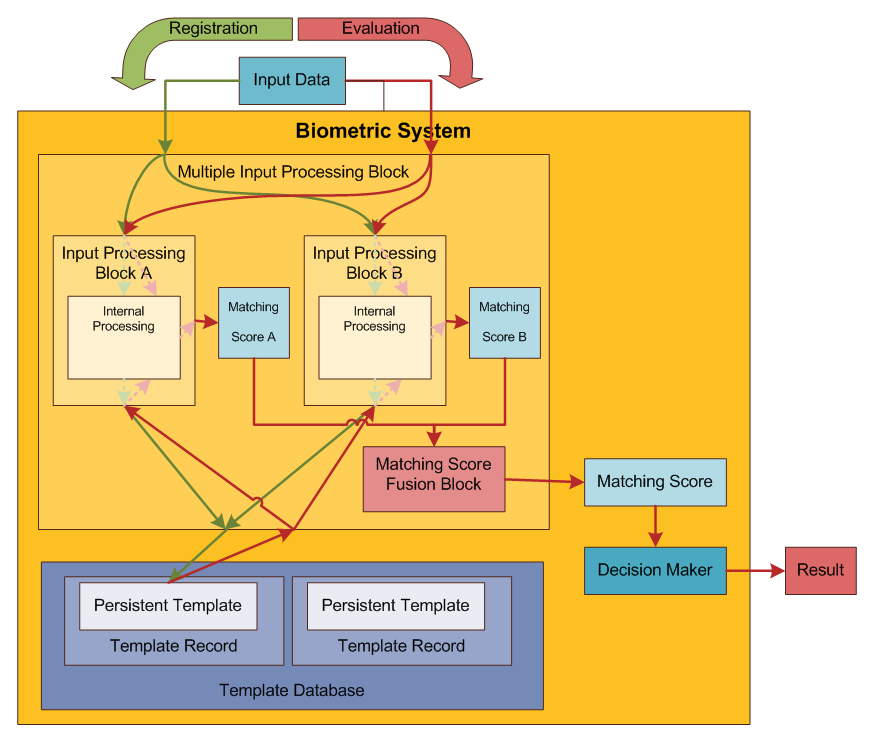
\includegraphics[width=12cm]{fig/fusion.eps}
	\caption{\label{fig:fusion} Podstata využitia viacerých vyhodnocovacích
	blokov\,--\,\emph{fusion}}
\end{figure}
\vfill
\vfill

\clearpage

\begin{figure}[ht!]
	\centering
	
\includegraphics[width=12cm]{fig/alg5.eps}
	\caption{\label{fig:alg5} Výsledky implementovaného algoritmu \emph{Alg5}}
\end{figure}

\clearpage
\subsection{Prehľad výsledkov algoritmov} \label{vysledky}

\begin{figure}[ht!]
	\centering
	
\includegraphics[width=12cm]{fig/all.eps}
	\caption{\label{fig:all} DET a ROC krivky všetkých implementovaných algoritmov}
\end{figure}

\clearpage
\section{Porovnanie s existujúcim nástrojom} \label{konalio}

Vzhľadom na slabé výsledky nami implementovaných algoritmov, sme porovnali
extrakciu žíl z prstov s existujúcim nástrojom.

Využili sme extraktor žíl prstu \cite{konalio}, ktorý prezentuje vo svojej práci
výborné výsledky. Nástroj je písaný v jazyku C++ a umožňuje detekciu prstu
a následnú extrakciu žíl prstu. Výsledky algoritmu je možné nájsť na obrázkoch
ukážky \ref{fig:test_orig}, kde je možné vidieť pôvodný obrázok
(\uv{\emph{initial image}}), obrázok s detekovanou oblasťou prstu
(\uv{\emph{finger region}}), extrahované žily z prstu (\uv{\emph{extracted
veins}}) a zmenšene extrahované žily z prstu stenšené na 1 pixel
(\uv{\emph{tracked veins}}).

Pri použití snímku z databáze, s ktorou sme pracovali pri analýze nami
implementovaných algoritmov, dochádzalo k neporovnateľne slabým výsledkom.
Detekcia prstu bola často úspešná, avšak detekcia žíl bola neúspešná.
Výsledky porovnávania potvrdzujú slabú kvalitu vstupných snímkov. Výsledky
porovnávania snímku z databáze je možné nájsť v ukážke \ref{fig:test_nas}.

\begin{landscape}
\begin{figure}[ht!]
	\centering
	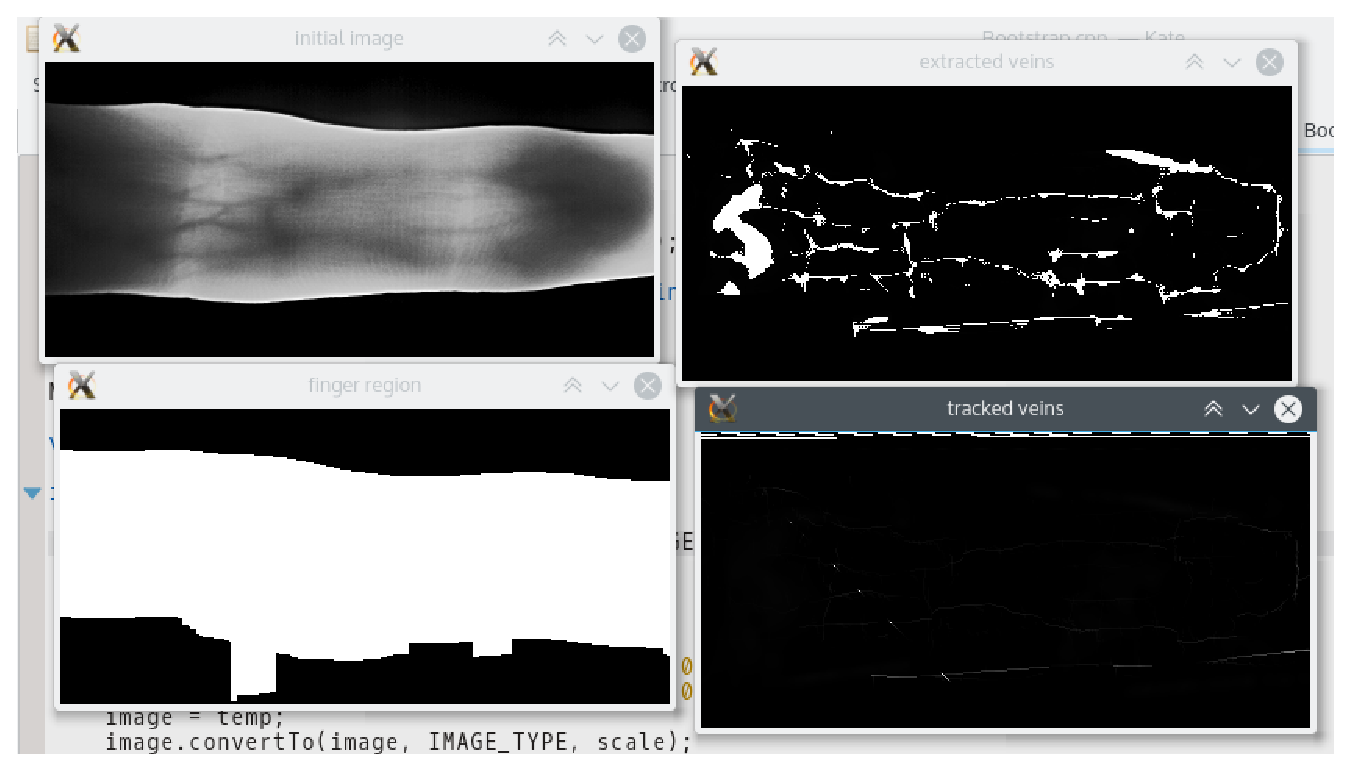
\includegraphics[width=27cm]{fig/test_orig.eps}
	\caption{\label{fig:test_orig} Práca porovnávaného algoritmu na snímkoch od autora porovnávaného algoritmu}
\end{figure}
\end{landscape}

\begin{landscape}
\begin{figure}[ht!]
	\centering
	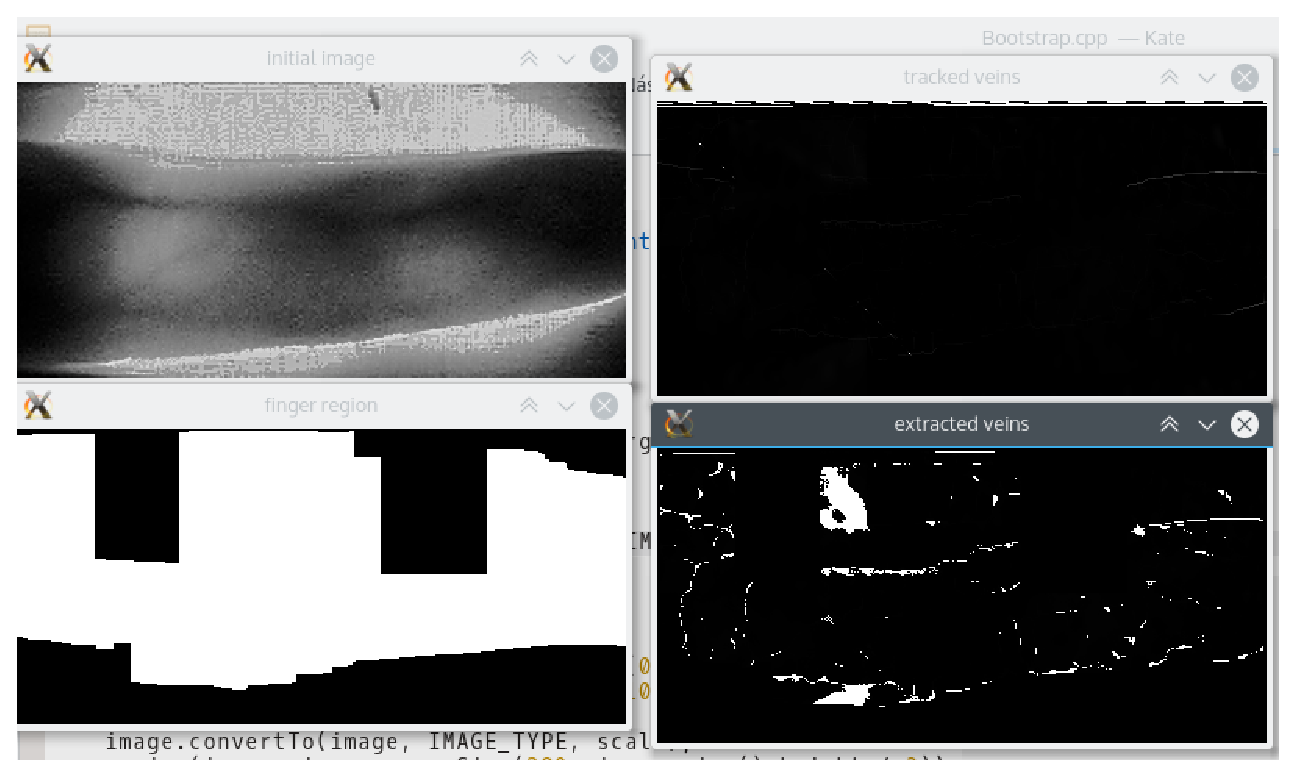
\includegraphics[width=27cm]{fig/test_nas.eps}
	\caption{\label{fig:test_nas} Práca porovnávaného algoritmu na našich snímkoch}
\end{figure}
\end{landscape}

\clearpage
\section{Záver} \label{zaver}

Bolo celkovo úspešne implementovaných 5 algoritmov pre rozpoznávanie ľudí na
základe žíl prstu. Algoritmy boli otestované a bola zvážená ich použiteľnosť.

Žiaľ, z implementovaných algoritmov ani jeden nedosahuje výsledky vhodné pre
prípadné nasadenie do biometrického systému. Hlavný problém vidíme v snímkoch zo
senzora, ktoré nedosahujú kvality vhodné pre použitie v reálnom biometrickom
systéme.

Hlavné možné zlepšenie vidíme vo využití lepšieho senzora. Snímky z lepšieho
senzora by podľa našeho uváženia mohli zlepšiť použiteľnosť implementovaných
algoritmov. Potvrdzuje to aj porovnanie s existujúcim nástrojom pre extrakciu
žíl prstu, ktorý nebol schopný extrahovať žily z používaných snímkov. Bez
kvalitnejších snímkov žiaľ nevieme získať lepšie výsledky.

\clearpage

\bibliographystyle{unsrt}
\bibliography{sample}
\addcontentsline{toc}{section}{Literatúra}
\begin{thebibliography}{99}

\bibitem{konalio}
	Kupidura P.,
	\emph{System for human identification based on finger vein pattern},
	[online: \url{https://github.com/konalio/FingerVeinRecognition}],
	[cite: 6.12.2015].

\bibitem{mahri}
	Nurhafizah M., Sundi S. A., Bakhtiar A. R.,
		\emph{Finger Vein Recognition Algorithm Using Phase Only Correlation},
	[online: \url{http

\end{thebibliography}

\end{document}

